\chapter{Physics Overview}
In order to give the proper context for the measurement shown in this thesis,  an overview of the physical theory relevant to the measurement is given in this chapter. We start with the SM (Standard Model of particle physics), narrow the focus down to QCD (Quantum Chromodynamics), and then narrow the focus even more to a specific state of matter governed by QCD known as QGP (Quark Gluon Plasma). Properties of QGP are discussed including energy loss and elliptic flow. A more comprehensive discussion on the topic of elliptic flow and small collision systems will be presented in Chapter 2.
\section{The Standard Model}
The SM is the best understanding of the fundamental building blocks reality and how they interact. The SM as we know it today has evolved over many years, including the unification of the electromagnetic and weak forces in the late 1960s. The present day SM includes four fundamental forces, listed in Table \ref{tbl:sm}, and the fundamental particles, listed in Figure \ref{fig:stnd_mdl_chart}.
\begin{table}[h!]
\caption{All four of the fundamental forces and the effective strengths of each relative to gravity. Gravity is not covered by the SM but is included for completeness.}
\begin{center}
%    \begin{tabular}{| l | l | l | | | | | | }
    \begin{tabular}{ccccc}
    \hline
    Force &Current Theory  & Relative Strength & Range [m] &  Force Carriers\\ \hline
    strong  & Quantum Chromodynamics (QCD) & $10^{41}$ & $10^-{15}$&  gluon\\
    electromagnetic &Quantum Electrodynamics (QED) & $10^{38}$ & infinity &  photon\\
    weak & Electroweak & $10^{25}$ &  $10^{-18}$ & $Z^0$,$W^{+/-}$\\
    gravity & General Relativity & 1 & infinity & graviton\\ \hline
    \end{tabular}
\end{center}
\label{tbl:sm}
\end{table}

\begin{figure}[!ht]
\begin{center}
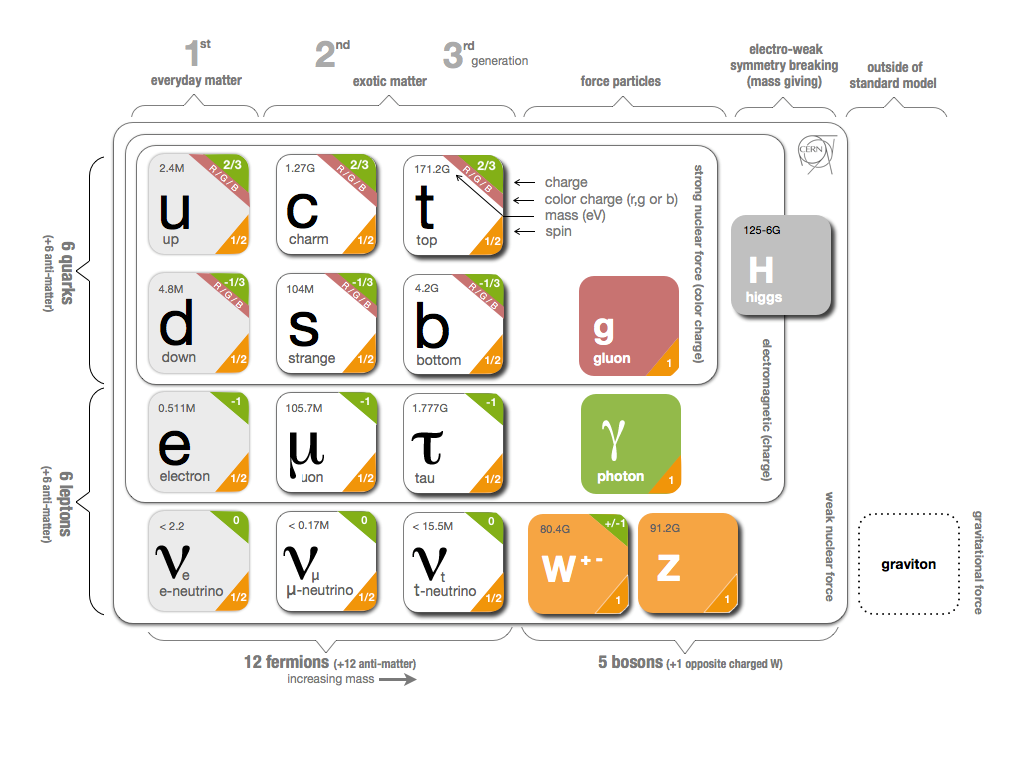
\includegraphics[width=0.65\linewidth]{figs/standard_model_chart.png}
\caption{The fundamental particles of the SM arranged to highlight flavor (horizontal) and charge (vertical) patterns among the particles. These are thought to be the smallest discrete pieces of matter which make up everything else in the universe ~\cite{PhysRevD.86.010001}.}
\end{center}
\label{fig:stnd_mdl_chart}
\end{figure}

The SM has the capability of making quantifiable predictions which have been shown to be in agreement with experimental measurements to many decimal places. The SM has endured decades of meticulous experimental testing without the need for major revisions, a notable exception being neutrino oscillations. The mathematical framework underpinning the SM is formally known as QFT (Quantum Field Theory) which combines the continuous nature of field physics with the discrete nature of quantum physics. 
The fundamental symmetries of the SM are given by the combination of the $SU(3)\times SU(2)\times U(1)$ groups as defined in group theory. Each symmetry group represents the symmetry of each of the fundamental forces in the SM such that $SU(3)$, $SU(2)$, and $U(1)$ represent the strong, weak, and electromagnetic forces respectively. As shown in table \ref{tbl:sm}, each of the fundamental forces has a quantized theory associated with it. The electromagnetic and weak forces combine into a single theory at high energy, known as the Electroweak Theory. No similar theory which has been experimentally verified has combined strong and electroweak upon writing of this thesis.

Any given interaction described by the SM starts with an initial set of particles, a series of interactions between those particles (which is represented by an exchange of virtual particles), and then a set of final state output particles. Experimentally, the only information available to the experimenter is the list of input particles and output particles. The in-between step of the interaction of the particles is where QFT is used. Theoretical physicists use QFT to calculate the probabilities of each possible interaction diagram given a set of input particles or a set of output particles or both. To complicate things, there are infinite possible interaction diagrams for any given set of inputs and outputs; however, there are always leading diagrams which have the highest probability of occurring. Generally the simpler the interaction diagram, the higher the probability.

In order to make predictions about physical systems dominated by the strong force, like the heavy ion collision systems studied in this thesis, we turn to QCD. 

\subsection{Quantum Chromodynamics}
Of the fundamental particles which make up the SM, the only seven which interact through the strong force are the six quarks and the gluon. 
These particles have a unique quantum number named color charge which can be one of three values referred to as
red (r), green (g), and blue (b), in an analogy to three colors commonly used to form the basis of light in the visible spectrum. Like the electric
charge in QED, each color has a negative value
 referred to as anti-red ($\overline{\text{r}}$), anti-green ($\overline{\text{g}}$), and anti-blue($\overline{\text{b}}$), making six possible states for the quantum number in total. Gluons have two color charge quantum numbers, one charge and one anti-charge. This fact means gluons interact with themselves, which produces two important effects in QCD: confinement and asymptotic freedom.

\begin{figure}[!ht]
\begin{center}
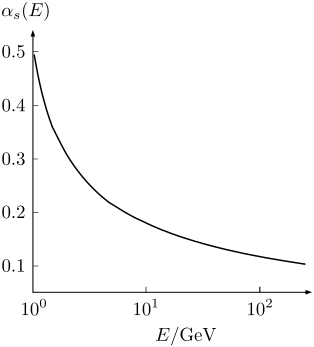
\includegraphics[width=0.45\linewidth]{figs/coupling_constant.png}
\caption{The strong coupling $\alpha_s$ as a function of energy of the square root of the energy or momentum transfer $Q$. ~\cite{Bethke2009}.}
\end{center}
\label{fig:coupling_plot}
\end{figure}

In QED, electromagnetic fields decrease with distance away from a point charge. This functional form allows electromagnetically bound states to separate.
However in QCD, the self interaction of the gluon means that as two quarks separate, the force between them grows proportionally to the distance between them. As a
quark-antiquark (q$\overline{\text{q}}$) pair separates, each quark in the pair has so much potential energy that quarks from the vacuum bind to each quark to form two new pairs. The outcome of this effect is that solitary quarks can never be observed in a vacuum, by the time we try to observe them they will have found another particle in the vacuum with which to bind. This means that quarks are confined to zero color charge (or color neutral) bound states. Color neutral bound states are defined as a color state and anti-color state  (ex. r$\overline{\text{r}}$, g$\overline{\text{g}}$, b$\overline{\text{b}}$),  known as mesons, or a tricolor state (ex. rgb or $\overline{\text{r}}\overline{\text{g}}\overline{\text{b}}$), known as baryons. The list of the two or three quarks which make up color neutral bound state are known as valence quarks. Valence quarks are quarks which determine the quantum number for the hadron in contrast to sea quarks which are q$\overline{\text{q}}$ pairs made from gluon annihilations and fill all the lower states. Quarks and gluons found in hadrons are known as partons, and partons carry a fraction of the hadron's total momentum $x$. Partons can have any momentum fraction of the total momentum, but it is most probable that valence quarks have one third of the total momentum where as gluons and sea quarks are more likely to have a much smaller momentum fraction. Figure \ref{fig:pdf_plot} shows measured parton distribution functions in the proton, illustrating the difference of the average $x$ for valence quarks in contrast to sea quarks.

\begin{figure}[!ht]
\begin{center}
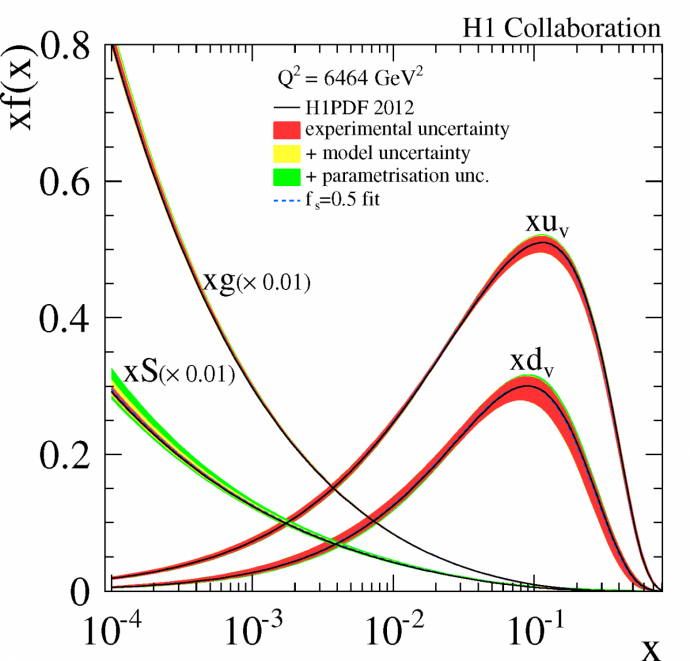
\includegraphics[width=0.45\linewidth]{figs/parton_distribution.png}
\caption{Parton distribution functions (PDF) of the the momentum fraction $x$ in the proton extracted from the data taken by the H1 Collaboration. The curves $xS$, $xg$, $xu_v$, and $xd_v$ correspond to PDFs of sea quarks, gluons, up valence quarks, and down valence quarks in the proton. The gluon $g$ and sea $S$ distributions are scaled by a factor 0.01. The uncertainties include experimental (inner) and model (middle) uncertainties and the parametrization variations (outer). ~\cite{Aaron2012}.}
\end{center}
\label{fig:pdf_plot}
\end{figure}

Color neutrality can arise from other combinations of quarks; from combinations of quarks and gluons; or even arrangements of gluons with no valence quarks. The first mentioned combinations are theoretical color neutral states of four or more quarks which have yet to be experimentally observed. The second and third mentioned combinations are known as exotic mesons or glueballs and there are experiments searching for their signatures.

Another related effect of the self-interaction of the gluon is known as the screening of bare color charges.  Once again it is helpful to compare to the familiar effects in QED. In QED, electrically charged pairs from the vacuum screen out the bare electric charge, causing the effective charge to decrease. This effect increases as the distance to the electric charge increases because there is a larger quantity of electrically charged pairs between the observer and the charge. Back to QCD, qq pairs produce the same effect, providing a screening effect on the bare color charge, however short-lived the bare color charges are. Further complications arise when the color-carrying gluon in turn creates an anti-screening effect, which is the larger of the two effects. As one approaches a solitary color charge, the density of gluons becomes so large that the strong force counter-intuitively grows weaker. These screening effects alter the strong coupling constant known as $\alpha_s$ which is proportional to the local strong force magnitude. Figure \ref{fig:coupling_plot}, which depicts the $\alpha_s$ as a function of energy scale, shows the reduction of $\alpha_s$ at large energies. This behavior is known as asymptotic freedom because the smaller $\alpha_s$ is, the more quarks can move freely. Thus, there is an energy threshold where the strong force is weak enough where perturbative calculations are valid. The ability to make valid perturbative calculations for QCD is important for being able to make any in-depth QCD calculations of complex systems. Apart from perturbative QCD calculations, lattice QCD is a non-perturbative approach which is formulated on a lattice of space-time points. Although lattice QCD calculations are computationally complex, physical phenomena such as quark confinement can be treated analytically.

In addition to understanding the unique effects of QCD, understanding the phases of QCD matter is important. Figure \ref{fig:qcd_phase} is a phase diagram for quark matter with temperature  and net baryonic density on the axes. The type of quark matter which makes up the elements of normal matter is found in the figure under the heading of ``Nuclear Matter" which is the state of quarks and gluons for complex, relatively stable bound states known as nuclei. The ``hadronic phase" indicates a state of quark matter where bound states of quarks form hadrons but those hadrons behave like a non-interacting gas. At very large baryonic density, the ``color superconductivity" phase is where the possible quantum states of quarks and gluons are so full that an example of such a state of matter is a neutron star. Finally, under extreme conditions of temperature and bayonic density, quarks may be deconfined and exist as solitary color charges in a plasma. This phase of matter, known as QGP (Quark-Gluon Plasma), provides a medium where screening effects are dominant and $\alpha_s$ becomes small enough to allow quarks and gluons to move with relative freedom. Although QGP has been observed by multiple experiments at RHIC (Relativistic Heavy Ion Collider) and LHC (Large Hadron Collider) facilities, the critical temperature at which the phase of quark matter is achieved is still unknown, although some recent experiments place the temperature at 170 MeV or 1.9$\times10^{12}$ kelvin, which is much hotter than the center of our sun~\cite{doi:10.1142/9789814689304_0031}.

\begin{figure}[!ht]
\begin{center}
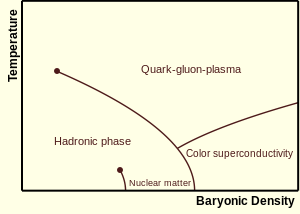
\includegraphics[width=0.55\linewidth]{figs/qcd_phase_diagram.png}
\caption{QCD phase diagram of with temperature on the y-axis and net baryonic density on the x-axis~\cite{Bhalerao:2014owa}.}
\end{center}
\label{fig:qcd_phase}
\end{figure}

Lattice QCD calculations have been done to examine the relationship of the number of massless degrees of freedom and the temperature of the medium as which provide insight in how QGP and the early universe transition into normal matter. Figure \ref{fig:lattice_degrees} shows a curve of a quantity inversely proportional to the number of massless degrees of freedom. As the temperature drops, the less massive particles annihilate and disappear from the thermal universe, reducing the degrees of freedom. The points on Figure \ref{fig:lattice_degrees_calc} are the numerical results from a lattice QCD calculation of the Equation of State (EoS). The y-axis for the points on this plot is the energy density divided the temperature to the fourth power $\frac{\epsilon}{T^4}$ which has been shown to be inversely proportional to the number of massless degrees of freedom~\cite{PhysRevD.81.054504}. It is noteworthy that the points increase around the transition indicating the disappearance of the degrees of freedom around the transition temperature of the medium.

\begin{figure}[!ht]
\begin{center}
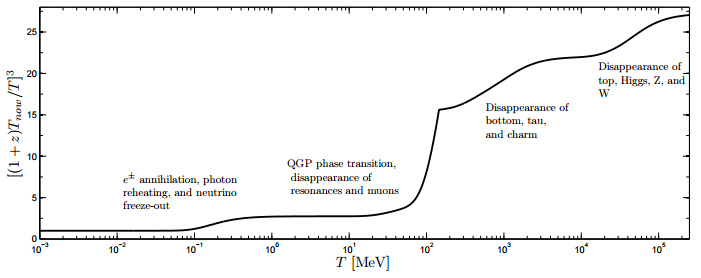
\includegraphics[width=0.55\linewidth]{figs/lattice_degrees_plot.PNG}
\caption{Disappearance of degrees of freedom through the evolution of the Universe in time
and how this affects the fractional drop of temperature compared to red-shift~\cite{1742-6596-509-1-012014}.}
\end{center}
\label{fig:lattice_degrees}
\end{figure}

\begin{figure}[!ht]
\begin{center}
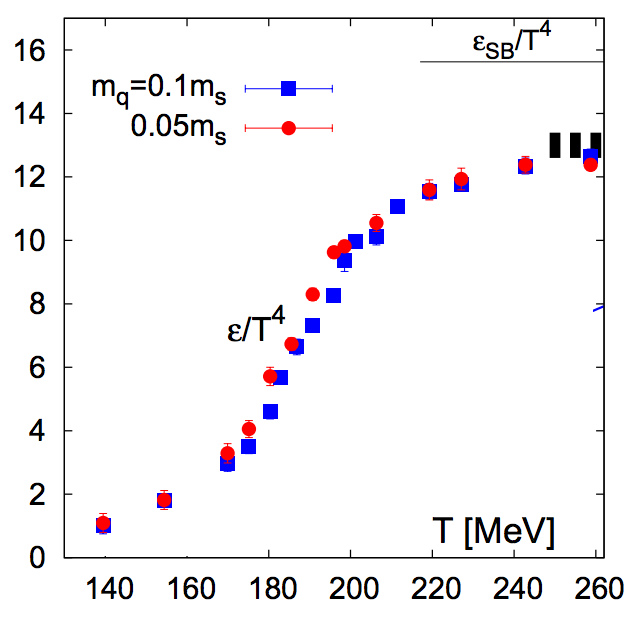
\includegraphics[width=0.55\linewidth]{figs/lattice_degrees_calculation.png}
\caption{The energy density $\epsilon$ divided by $T^4$ vs temperature $T$ at the physical value of the light quark mass~\cite{PhysRevD.81.054504}.}
\end{center}
\label{fig:lattice_degrees_calc}
\end{figure}

\section{Quark Gluon Plasma}
QGP is a new state of matter created in science laboratories and is thought to be the same as the entire early universe approximately one microsecond after the big bang ~\cite{RAFELSKI2013155}. Thus, studying QGP and its properties in the laboratory can help cosmologists understand the state of the early universe.

The idea of hot hadronic matter was developed in the early 1950s by various physicists including Enrico Fermi~\cite{Fermi01071950}. This concept of applying statistical and hydrodynamical models to a strongly interacting particle ensemble ultimately evolved into the theory of QGP. Since then, systematic studies of hot hadronic matter systems have produced a greater understanding of the state of matter hypothesized to be QGP and contributed to its approximate location on the nuclear matter phase diagram in Figure \ref{fig:qcd_phase}. Many unique properties about this new state of matter have been discovered: for example, QGP behaves like a nearly perfect fluid and is opaque to color charges~\cite{Akiba:2015jwa}. Enough research has been done to assemble a probable timeline of how the QGP evolves.

\subsection{QGP Evolution Timeline}
The timeline overview of QGP as made in the laboratory always begins with a high-energy heavy ion collision (Au-Au for example), thus the QGP timeline is embedded in the laboratory timeline. As is the case with all SM interactions, the beginning of QGP starts with initial state observable particles and ends with final state observable particles, although the final state particles may have been produced at different points during the QGP evolution. Although only lasting $10^{-23}$ seconds or $10 fm/c$, several distinct stages occur during this time period and long after the evolution has ceased the final state particles are detected in the experiment one quadrillion QGP lifetimes or one nanosecond later.

At the moment when heavy ions collide relativistically ($\tau$=0), they are length contracted down to flat disks in the lab frame, as seen in Figure \ref{fig:qgp_timeline}. Then, the initial geometry resulting from the shape of the collision overlap region and fluctuations within the nuclei are transformed into the initial energy density of the medium ($\tau$ $\approx$ 1 fm/c). At that moment, the hot hadronic matter is thought to be made up of deconfined quarks and gluons in thermal equilibrium, otherwise known as QGP. The system then evolves hydrodynamically, expanding along the pressure gradients present in the initial energy density. At a certain point during this expansion, the medium has cooled down enough in order to form baryons and mesons out of the quark gluon soup in a process known as hadronization. It is important to note that the medium is still in thermal equilibrium at this point although it is no longer known as QGP, instead it is known as hadron gas. Once the medium has cooled down and expanded sufficiently, kinetic freeze-out occurs and the hadron gas becomes a group of particles which have ceased self-interaction ($\tau$ $\approx$ 10 fm/c). It is this group of final state particles which can be detected much later ($\tau \approx 10^{15}$ fm/c). Although detectable particles escape the medium at all times, the vast majority of particles detected are decoupled at kinetic freeze-out. 

Even though all of these phases are of interest to the study of QGP, of particular interest to QGP researchers is the thermal equilibrium phase when the QGP state is first achieved. It is during this phase where quarks are deconfined, the only time or place in the universe where this occurs. In this environment, features of QCD can be studied, such as how color charges experience energy loss and to what degree is collective behavior observed. 

As is referred to in Figure ~\ref{fig:qgp_timeline}, many types of particles are emitted during the QGP evolution, some of which are emitted before the kinetic freeze-out time. The most common type of particle produced from QGP collisions are baryons and mesons made of up, down, and strange quarks (pions, Kaons, and nucleons), which are in abundant supply during and after the collision. Another type of particle produced from these collisions are photons. QGP being an extremely hot ball of matter, blackbody radiation in the form of thermal photons are emitted and their spectrum can be used to estimate the temperature of the medium. These thermal photons escape the medium due to their lack of interaction with the strong force. Heavy quarks are produced primarily from initial hard parton-parton scatterings, ``hard" meaning here that there is a large momentum transfer in the collision. These heavy quarks, such as bottom or charm quarks, often fragment into a shower of less massive particles known as jets as they propagate through space.
% maybe add lepton production later

\begin{figure}[!ht]
\begin{center}
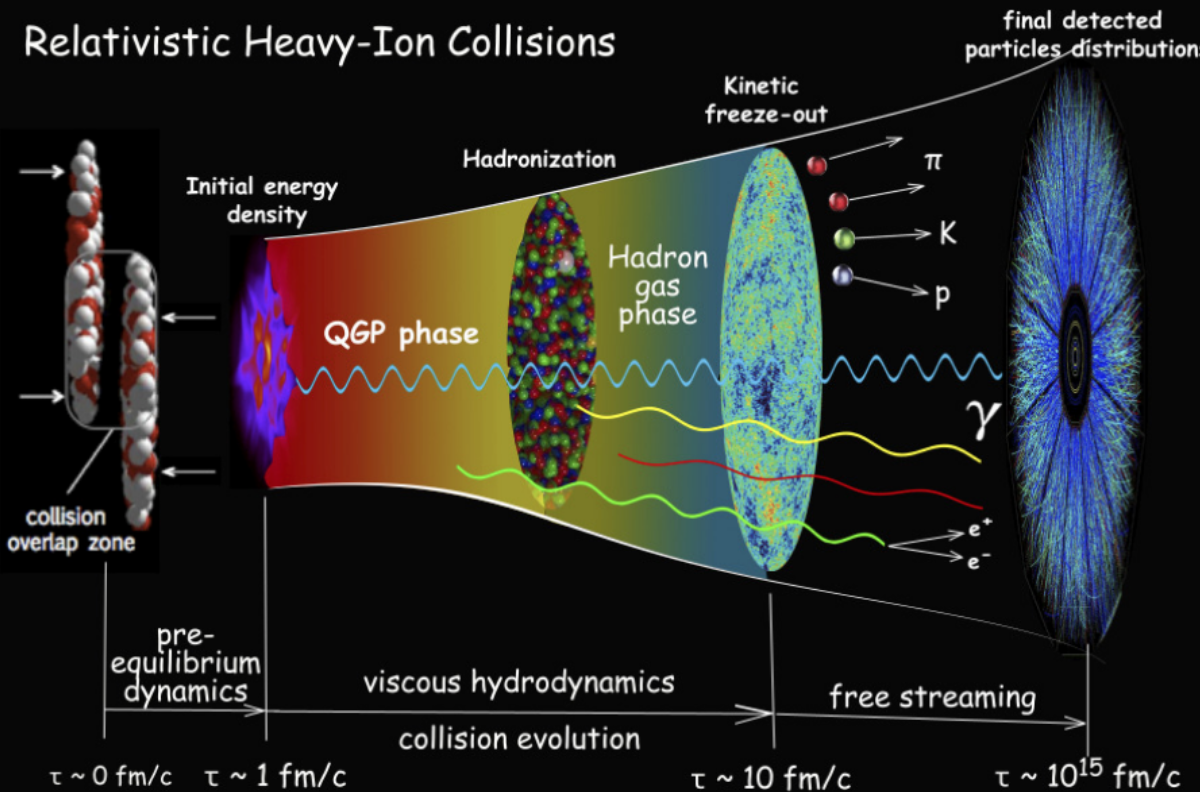
\includegraphics[width=0.78\linewidth]{figs/qgp_evolution_timeline.png}
\caption{Relativistic heavy ion collision evolution timeline starting. Three distinct phases and their times are shown as well as the particles produced~\cite{Heinz:2013wva}.}
\end{center}
\label{fig:qgp_timeline}
\end{figure}

\subsection{Emergent Properties of the QGP}
Now that the foundation of the QGP timeline has been established, properties of the medium can be discussed in context. Up to this point in this document, the label of QGP has been applied to state of matter produced from heavy ion collisions, but what evidence is there that this state of matter is a strongly coupled medium made of deconfined quarks and gluons?

Taking into account that the field of high-energy heavy ion collision physics is still evolving, several measured properties of this state of matter have come together to make QGP the prevailing explanation. Among the best observations indicating QGP are particle energy loss and elliptic flow. The observation of hadrons at large $p_T$ measured at much lower yields than expected imply that the hadrons are experiencing energy loss when interacting with a strongly coupled medium.  An elliptic symmetry in the angular distribution of final state particles when viewed along the axis of collision has been observed. The translation of initial geometry into long-range angular correlations indicates collectivity in a strongly coupled medium.

%The observation of a severe reduction in the number of expected J/$\psi$ particles matches a prediction that a strongly coupled medium with a temperature above the Hagedorn temperature will melt J/$\psi$ particles.

\subsubsection{Particle Energy Loss}
In order to study a new medium such as QGP, it is useful to measure things about the QGP relative to a more well known collision system such as p+p. By measuring the relative number of hadrons produced at various transverse momentums in both p+p and heavy ion collisions, QGP medium effects can be teased out.

After the quarks are produced in p+p collisions, they will hadronize and freely travel to the experiment's detector. In heavy ion collisions, the quarks propagate through, and interact
with, the QGP, exchanging energy and momentum with the medium along the way. The effect of energy loss on these quarks will modify their yield relative to the yield in p+p collisions.The nuclear modification factor $R_{AA}$ is the observable used is to quantify this modification which is defined for a given particle as:

\begin{equation}\label{eqn:raa}
 R_{AA}(p_T) = \frac{dN_{AA}/dp_T}{\left<N_{coll}\right>\times dN_{pp}/dp_T},
\end{equation}
where $dN_{AA}/dp_T$ and $dN_{pp}/dp_T$ is the yield of a given particle vs $p_T$ in heavy ion collisions and p+p collisions respectively and $N_{coll}$ is the average number of binary collisions for a given class of events. In summary, the $R_{AA}$ is a ratio for how many particles are produced for the same system with a normalization factor of $N_{coll}$ to account for the differences in system size. The $\left<N_{coll}\right>$ value is usually determined using Monte Carlo Glauber simulations and will be discussed in more detail in Chapter 2. If the particles do not interact with the medium, the $R_{AA}$ should be equal to 1.0. A value above 1.0 is interpreted as an enhancement of particles and a value below 1.0 is interpreted as a suppression of particles. 

Figure \ref{fig:RAA_plot} shows a significant suppression in the $R_{AA}$ vs $p_T$ (transverse momentum) of $\pi^0$ mesons produced in Au+Au collisions at $\sqrt{s_{NN}}$ = 200 GeV at RHIC for large and small sized QGP events, 0-10$\%$ central and 80-92$\%$ central events respectively (centrality will be discussed in Chapter 2). This large suppression across all  $p_T$ of the $\pi^0$ for large-sized events as compared to small-sized events indicate energy loss of quarks due to the medium, which is consistent with a strongly coupled  medium.

\begin{figure}[!ht]
\begin{center}
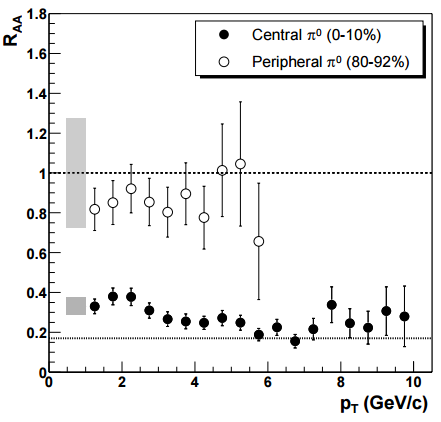
\includegraphics[width=0.6\linewidth]{figs/raa_pi0_aa_cent_periph.png}
\caption{The $R_{AA}$  vs $p_T$ of $\pi^0$ mesons produced in Au+Au collisions at $\sqrt{s_{NN}} = 200 GeV$ at RHIC for two different collision multiplicity classes. ~\cite{PhysRevLett.91.072303}}
\end{center}
\label{fig:RAA_plot}
\end{figure}
\clearpage
%\subsubsection{J/$\psi$ Melting}

\subsubsection{Collective Flow and Azimuthal Anisotropy}
Another signal of a strongly coupled medium is collective behavior amongst the constituent particles which make up the medium. By analyzing patterns in the spray of particles emitted from heavy ion collisions, systematic effects can be determined. Nominally there should be no preference in direction for final state particles from a heavy ion collision, the presence of such a preference can indicates correlations among the particles in the medium which can be measured by looking at the azimuthal anisotropy.

Consider the collision of two heavy nuclei as depicted in Figure ~\ref{fig:flow_diagram_cart}. The overlap region between the two nuclei form an almond shaped region oriented to the plane of the initial collision geometry. After the collision the two nuclei remnants (the blue shapes) no longer participate and the yellow overlap region forms the QGP medium and starts to expand. This energy density distribution gives rise to a larger pressure gradient in the shorter direction rather than the longer direction. The larger the pressure gradient, the more momentum the particles will gain once the medium finishes evolving. This variation in the momentum of final state particles produces systematic effects in the azimuthal (relative to the collision axis) distribution of particles. Therefore, by measuring the azimuthal anisotropy of the final state particles, long-range angular correlation like those present in this in Figure \ref{fig:flow_diagram_cart} can be measured. The initial state collision geometry being transformed into final state momentum anisotropy indicates collective behavior and elliptical flow of the particles.

\begin{figure}[!ht]
\begin{center}
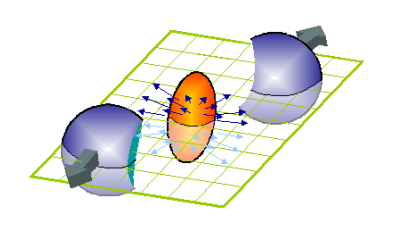
\includegraphics[width=0.5\linewidth]{figs/flow_diagram_cartoon.png}
\caption{A diagram of a heavy ion collision. The blue shapes are the two colliding nuclei and the elliptical yellow shape is the collision overlap region which forms the medium. In the next instant of time the two nuclei would travel father along the collision axis (into and out of the page) and the medium would expand along the direction of the arrows~\cite{Qin:2015nma}.}
\end{center}
\label{fig:flow_diagram_cart}
\end{figure}

In order to quantify the azimuthal anisotropy, the final state particle distribution is Fourier transformed:
\begin{equation}\label{eqn:dndphi}
  C(\Delta\phi) \propto 1 + \sum_{n=1}2 v_{n}\cos(n\Delta\phi]) 
\end{equation}
where $C(\Delta\phi)$ is the correlation function defined by the distribution of the differences between the azimuth of particles from the event relative to other particles in the same event, and $v_n$ are flow coefficients. The flow coefficients $v_n$ are proportional to the degree of anisotropy for each harmonic order $n$. A $v_n$ of 0.0 would indicate there is no azimuthal anisotropy. In addition to measuring the $v_n$ for various systems, a relativistic hydrodynamic calculation can be compared to the data. Figure \ref{fig:vn_aa_hydro} shows $v_n$ vs $p_T$ for both RHIC and LHC energy heavy ion collisions for mid-peripheral events, such as those depicted in Figure \ref{fig:flow_diagram_cart}. The substantial agreement with hydrodynamic calculations  curves indicates a medium which flows.

\begin{figure}[!ht]
\begin{center}
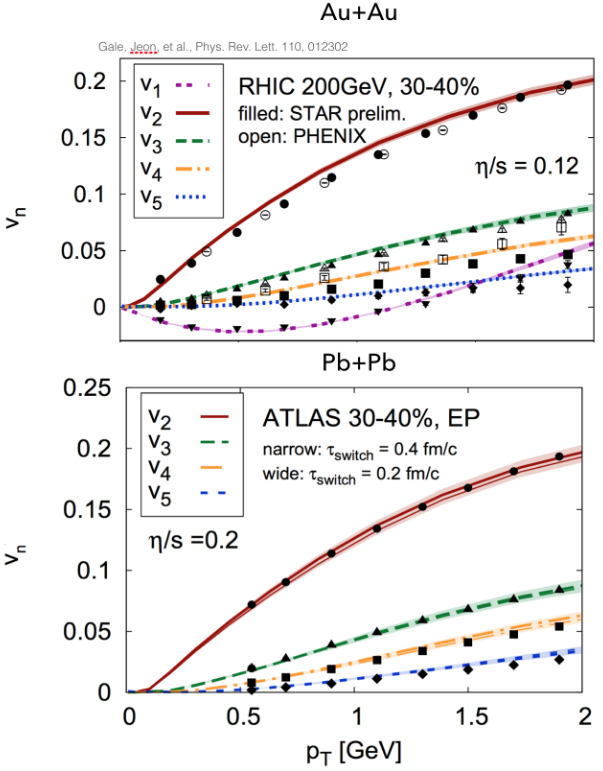
\includegraphics[width=0.65\linewidth]{figs/vn_aa_pbpb_hydro.PNG}
\caption{$v_n$ vs $p_T$ for RHIC Au+Au $\sqrt{s_{NN}}$ = 200 GeV and for LHC Pb+Pb $\sqrt{s_{NN}}$ = 2.76 TeV for mid-peripheral events for harmonic orders n up to five. The colored curves are the hydrodynamic calculations. The $\eta/s$ is the viscosity parameter used in the calculations~\cite{PhysRevLett.110.012302}.}
\end{center}
\label{fig:vn_aa_hydro}
\end{figure}

All of the discussion and results shown in this section have been referring to large collision systems such as Au+Au or Pb+Pb. Small collision systems such as p+Au, d+Au, or p+p were thought to be too small to produce QGP, and thus were ideal as the control experiment to measure background effects of cold nuclei which may obscure the true signal of QGP. However, recent results have shown that small collision systems show signs of QGP formation. Chapter 2 will delve into small collision systems properties and measurements, as well as give a more in-depth discussion in calculating initial conditions and flow coefficients.
